%%%% METRICS AND MODELS %%%%
\chapter{Review of existing auditory metrics and models}\label{chap:04_Auditory_Models}
In this chapter, we review some existing auditory metrics and models.
As will be discussed in \chapref{chap:05_Proposed_Models}, some of these metrics and models may be more or less suitable for evaluating and comparing navigational techniques.
Nevertheless, the metrics and models presented here comprise a core set of tools on which subsequent models and analyses will be based.

While in some cases the metrics described below provide an absolute measure of the desired quality (e.g., sound level or localization direction), we are often more interested in obtaining a relative measure of that quality.
For example, coloration is rarely measured in an absolute sense, but instead as a perceptible difference induced via some process.
Consequently, some metrics are computed using both a \textit{test signal} (i.e., the estimated ambisonics impulse response for the listening position after processing by some navigational method) and a \textit{reference signal} (i.e., the ambisonics impulse response captured directly at the listening position).

\section{Level metrics}\label{sec:04_Auditory_Models:Level_Metrics}
Here, we describe a numerical measure of sound level (or amplitude), which aims to predict (or at least correlate with) perceived loudness.

%% Audible Energy
\subsection{Mean audible energy (\texorpdfstring{$\lambda$}{lambda})}\label{sec:04_Auditory_Models:Audible_Energy}
We define the \textit{mean audible energy} (MAE), $\lambda$, of an ambisonics signal as the average energy of the zeroth-order term across a set of critical bands,%
\footnote{Roughly speaking, a \textit{critical band} refers to the bandwidth of the effective auditory filter created by the cochlea, within which a stronger second tone will mask the perception of a weaker first tone \citep[chapter 3]{Moore2013}.}
 i.e.,
\begin{equation}\label{eq:04_Auditory_Models:Mean_Audible_Energy}
\lambda = 10 \log_{10} \left( \frac{1}{N_b} \sum_{c = 1}^{N_b} \frac{\displaystyle \int_{-\infty}^\infty |H_\Gamma(f;f_c)| |A_0(f)|^2 df}{\displaystyle \int_{-\infty}^\infty |H_\Gamma(f;f_c)| df} \right),
\end{equation}
where $|\cdot|$ again denotes the absolute value of the argument and $H_\Gamma(f;f_c)$ is the transfer function of a gammatone filter%
\footnote{In this work, we used the gammatone filters implemented in the large time-frequency analysis toolbox (LTFAT) for MATLAB \citep{LTFATURL}.} (which approximates critical bands) with center frequency $f_c$ for $c \in [1, N_b]$, for a set of ERB-spaced (equivalent rectangular bandwidth) center frequencies \citep{GlasbergMoore1990} spanning the range $f \in [50~\text{Hz}, 21~\text{kHz}]$.
Magnitude responses of the first four of these filters are shown in \figref{fig:04_Auditory_Models:Gammatone_Filters}.
As shown in that plot, these filters effectively act as narrow band-pass filters, and the spacing between adjacent filters decreases with increasing frequency (when plotted on a logarithmic axis) due to the ERB spacing.
Due to these filters, the summand in \eqnref{eq:04_Auditory_Models:Mean_Audible_Energy} approximately represents the power spectrum of a signal reaching the cochlea, as defined by \citet[Eq.~(5.12)]{Salomons1995PhD}.

\begin{figure*}[t]
    	\centering
    	\begin{subfigure}[b]{0.49\textwidth}
        		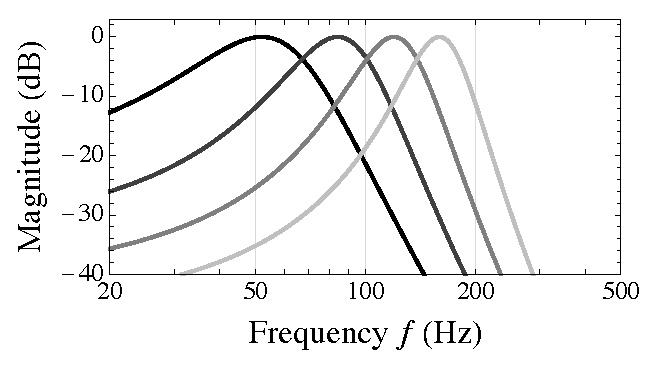
\includegraphics[width=\textwidth]{04_auditory_models/figures/gammatone_mag.eps}
        		\caption{Gammatone filters, $H_\Gamma$}
        		\label{fig:04_Auditory_Models:Gammatone_Filters}
    	\end{subfigure}
	\hfill
    	\begin{subfigure}[b]{0.49\textwidth}
        		\includegraphics[width=\textwidth]{04_auditory_models/figures/patterson_mag.eps}
        		\caption{Patterson's filters, $H_\text{P}$}
        		\label{fig:04_Auditory_Models:Patterson_Filters}
    	\end{subfigure}
	
	\caption[Magnitude responses of gammatone filters and Patterson's filters.]{
	Magnitude responses of gammatone filters (left panel) and Patterson's filters (right) for the first four ERB-spaced center frequencies increasing from approximately 50~Hz.}
	\label{fig:04_Auditory_Models:Auditory_Filters}
\end{figure*}

We further define the level error given in dB by
\begin{equation}\label{eq:04_Auditory_Models:Audible_Energy_Difference}
e_\lambda = \tilde{\lambda} - \lambda,
\end{equation}
where $\lambda$ is the MAE for a reference signal and $\tilde{\lambda}$ is that for a test signal.

\section{Coloration metrics}\label{sec:04_Auditory_Models:Coloration_Metrics}
Generally, we use the term \textit{spectral coloration} to refer to any changes in the spectral content of a signal, for instance due to the application of a filter whose magnitude response is not constant.
However, as not all colorations are equally audible, metrics which mimic auditory filtering processes offer more perceptually-relevant estimates of colorations.
Here, we review five metrics that all aim to quantify such colorations.
For several of these metrics, we further define the \textit{spectral range}, given by
\begin{equation}\label{eq:Spectral_Range}
\rho_S = \max_c S(f_c) - \min_c S(f_c),
\end{equation}
and the \textit{spectral deviation}, given by
\begin{equation}\label{eq:Spectral_Deviation}
\sigma_S = \sqrt{\frac{1}{N_b} \sum_{c = 1}^{N_b} \left( S(f_c) - \overline{S} \right)^2},
\end{equation}
where $S$ is some metric (specified in dB, unless stated otherwise) and $\overline{S}$ is its average over all frequency bands.
For these metrics, we use the frequency range $f \in [f_\text{L}, f_\text{U}]$ with $f_\text{L} = 50$~Hz and $f_\text{U} = 21$~kHz, as recommended by~\citet{Boren2015}.

%% Scharer's ABSE
\subsection{Auditory band spectral error (\texorpdfstring{$\eta$}{eta})}\label{sec:04_Auditory_Models:Coloration_Metrics:ABSE}
The \textit{auditory band spectral error} (ABSE), adapted from \citet[Eq.~(9)]{ScharerLindau2009}, is given by
\begin{equation}\label{eq:ABSE}
\eta(f_c) = 10 \log_{10} \left( \frac{\int |H_\Gamma(f;f_c)| |\tilde{A}_0(f)|^2 df}{\int |H_\Gamma(f;f_c)| |A_0(f)|^2 df} \right),
\end{equation}
where $A_0$ and $\tilde{A}_0$ are the zeroth-order terms of the reference and test (respectively) ambisonics transfer functions and integration is taken over all frequencies.
For this and other coloration metrics requiring an auditory filter bank, we use ERB-spaced center frequencies \citep{GlasbergMoore1990} spanning the range $f \in [f_\text{L}, f_\text{U}]$ and denoted $f_c$ for $c \in [1, N_b]$.
In this case, we define the spectral range and deviation of the ABSE: $\rho_\eta, \sigma_\eta$, respectively.

 %% Boren's Epk and En
\subsection{Peak and notch errors (\texorpdfstring{$E_{\text{pk}}, E_\text{n}$}{Epk, En})}\label{sec:04_Auditory_Models:Coloration_Metrics:Epk}
The \textit{peak and notch errors} ($E_{\text{pk}}, E_\text{n}$) were defined by \citet{Boren2015}
and essentially quantify the average peak (or notch) height (depth) in a frequency response over a certain frequency range.
First, the difference (in dB) is computed between finely- and coarsely-smoothed versions of the the normalized free-field transfer function $\tilde{A}_0(f)/A_0(f)$, i.e.,
\begin{equation}
D(f) = 20 \log_{10} \left( \frac{ \mathcal{S}\left( \left| \tilde{A}_0(f)/A_0(f) \right| ; 1/48 \right) }{ \mathcal{S}\left( \left| \tilde{A}_0(f)/A_0(f) \right| ; 1 \right) } \right),
\end{equation}
where $\mathcal{S}(X; B)$ denotes fractional-octave smoothing applied to the spectrum $X$ with smoothing bandwidth $B$ octaves.
Here, we used the fractional-octave smoothing method of \citet{Tylka2017}, reproduced in \apxref{chap:A3_Smoothing_Weights}.

The peak- and notch-finding algorithms described by \citeauthor{Boren2015} are then applied to find the frequencies $f_1^\uparrow, f_2^\uparrow, \dots f_{N_\text{pk}}^\uparrow$ of all $N_\text{pk}$ spectral peaks and $f_1^\downarrow, f_2^\downarrow, \dots f_{N_\text{n}}^\downarrow$  of all $N_\text{n}$ spectral notches in the range $f \in [f_\text{L}, f_\text{U}]$.
The peak and notch errors are then given by \citep[Eq.~(1)]{Boren2015}
\begin{equation}
E_\text{pk} = \frac{\sum_{j = 1}^{N_\text{pk}} D(f_j^\uparrow)}{3 \log_2 (f_\text{U}/f_\text{L})}
\quad\quad\text{and}\quad\quad
E_\text{n} = \frac{\sum_{j = 1}^{N_\text{n}} (-D(f_j^\downarrow))}{3 \log_2 (f_\text{U}/f_\text{L})},
\end{equation}
respectively.
Note that, since $D$ is given in dB, the negative sign in the second equation typically ensures that both metrics are positive-valued.

%% Kates' CS
\subsection{Central spectrum (CS)}
The \textit{central spectrum} (CS) was defined by \citet{Kates1984} for use as a metric for comparing loudspeaker responses.
Consequently, it may be employed using only the free-field transfer functions of the test and reference signals.
Essentially, the metric is computed as the sum of the Fourier coefficients and critical band energies of a time-weighted autocorrelation of the input signal (see the original paper for details).
We then compute the difference (in dB) between the central spectra for the test and reference signals, given by
\begin{equation}
e_\text{CS}(f_c) = \widetilde{\text{CS}}(f_c) - \text{CS}(f_c).
\end{equation}
As done for the ABSE, we define the spectral range and deviation of the CS: $\rho_{e_\text{CS}}, \sigma_{e_\text{CS}}$, respectively.

%% Pulkki's CLL
\subsection{Composite loudness level (CLL)}\label{sec:04_Auditory_Models:Coloration_Metrics:Pulkki_CLL}
The \textit{composite loudness level} (CLL) spectrum was defined by \citet[section 1.1]{Pulkki1999} to give an estimate of perceived loudness.
Computing the CLL requires binaural impulse responses, which we compute using \eqnref{eq:02_Acoustical_Theory:PW_Quadrature_Binaural}.
The CLL spectrum is then computed as the sum of the two ears' loudness level spectra, each of which are given in phons%
\footnote{The \textit{phon} is a unit of perceived loudness, and is related to dB SPL via the equal-loudness contours originally described by \citet{FletcherMunson1933}.
Similar to dB, a change in perceived loudness is computed via a difference of values in phons.}
and found via a gammatone filter bank, half-wave rectification, low-pass filtering, and time-averaging of the signal energy in each band (see the original paper for details).
We then compute the difference (in phons) between the CLL spectra for the test and reference samples, given by
\begin{equation}\label{eq:04_Auditory_Models:Pulkki_CLL}
e_\text{CLL}(f_c) = \widetilde{\text{CLL}}(f_c) - \text{CLL}(f_c).
\end{equation}
We then define the spectral range and deviation of the CLL: $\rho_{e_\text{CLL}}, \sigma_{e_\text{CLL}}$, respectively.

%% Wittek's SA
\subsection{Internal spectrum (IS)}\label{sec:04_Auditory_Models:Coloration_Metrics:Wittek_IS}
\citet{Wittek2007} adapted the \textit{internal spectrum} (IS) defined by \citet[chapter 5]{Salomons1995PhD} in order to define so-called \textit{spectral alterations}.
These spectral alterations are computed as the difference (in dB) between the internal spectra for the test and reference signals, given by
\begin{equation}
e_\text{IS}(f_c) = \widetilde{\text{IS}}(f_c) - \text{IS}(f_c).
\end{equation}
According to \citet[section 3.2.5]{Wittek2007}, the IS for each signal is given as the average of the binaural power spectra, i.e.,
\begin{equation}
\text{IS}(f_c) = 10 \log_{10} \left( \frac{P^\text{L}(f_c) + P^\text{R}(f_c)}{2} \right).
\end{equation}
Here, $P^{\text{L},\text{R}}$ are the binaural power spectra after critical-band filtering, given by \citep[Eq.~(5.12)]{Salomons1995PhD}
\begin{equation}
P^{\text{L},\text{R}}(f_c) = \frac{\displaystyle \int_{-\infty}^\infty |H_\text{P}(f;f_c)| |\psi^{\text{L},\text{R}}(f)|^2 df}{\displaystyle \int_{-\infty}^\infty |H_\text{P}(f;f_c)| df},
\end{equation}
where $H_\text{P}(f;f_c)$ are Patterson's auditory filters (which are very similar in magnitude response to gammatone filters, as shown in \figref{fig:04_Auditory_Models:Auditory_Filters}) as specified by \citet[Eq.~(5.9)]{Salomons1995PhD} and $\psi^{\text{L},\text{R}}$ are the binaural transfer functions, given by the Fourier transform of the binaural impulse responses from \eqnref{eq:02_Acoustical_Theory:PW_Quadrature_Binaural}.
Again, we define the spectral range and deviation of the IS: $\rho_{e_\text{IS}}, \sigma_{e_\text{IS}}$, respectively.
Note that $\rho_{e_\text{IS}}$ is precisely equivalent to the $A_0$-measure defined by \citet[section 3.2.6]{Wittek2007}, which is based on the $A_0$-criterion defined by \citet[section 5.4]{Salomons1995PhD}.
Additionally, $\sigma_{e_\text{IS}}$ is essentially equivalent to the ``spectral deviation'' described by \citet[section 3.2.6]{Wittek2007}.

\section{Localization models}\label{sec:04_Auditory_Models:Localization_Models}
Generally, we use the term \textit{source localization} to refer to the perceived direction of a sound source relative to a listener.
Here, we review two well-established primitive localization vectors and describe two more sophisticated localization models.
For a predicted localization direction $\hat{\nu}$ (computed at the position of the listener), the localization error $e_\nu$ is given by
\begin{equation}\label{eq:04_Auditory_Models:Localization_Error}
e_\nu = \cos^{-1} \left( \hat{\nu} \cdot \hat{s}_0{}' \right),
\end{equation}
where $\hat{s}_0{}'$ is the direction of the source relative to the listener, found by normalizing the vector $\vec{s}_0{}' = \vec{s}_0 - \vec{r}_0$.

%% Gerzon's Localization Vectors
\subsection{Velocity and energy vectors (\texorpdfstring{$\vec{\nu}_{\text{V}}, \vec{\nu}_{\text{E}}$}{vV, vE})}\label{sec:04_Auditory_Models:Localization_Vectors}
To predict the localization of sound in multichannel playback systems, \citet{Gerzon1992} defines two localization metrics: the velocity and energy vectors.
Note that these definitions assume that the loudspeakers are equidistant from the listening position, such that the signals all arrive coincidentally.

The velocity vector is used to predict localization due to interaural time differences at low frequencies ($<700$~Hz) and is given by \citep{Gerzon1992}
\begin{equation}\label{eq:04_Auditory_Models:Velocity_Vector}
\vec{\nu}_{\text{V}}(f) = \textrm{Re} \left\{ \frac{ \sum_q G_q(f) \hat{v}_q}{ \sum_q G_q(f)} \right\},
\end{equation}
where $\text{Re} \left\{ \cdot \right\}$ denotes taking the real part of the argument, $G_q$ is the complex-valued, frequency-dependent ``gain'' of the $q^{\text{th}}$ source, and $\vec{v}_q$ is the position of that source.
The energy vector is used to predict localization due to interaural level differences at higher frequencies (500~Hz -- 5~kHz) and is given by \citep{Gerzon1992}
\begin{equation}\label{eq:04_Auditory_Models:Energy_Vector}
\vec{\nu}_{\text{E}}(f) = \frac{ \sum_q |G_q(f)|^2 \hat{v}_q}{ \sum_q |G_q(f)|^2}.
\end{equation}
The directions of these vectors indicate the expected localization direction and their magnitudes indicate the quality of the localization.
Ideally, the vectors should have a magnitude equal to unity and point in the direction of the virtual source.

%% Stitt's Localization Model
\subsection{Precedence-effect-based energy vector (\texorpdfstring{$\vec{\nu}_{\text{PE}}$}{vPE})}\label{sec:04_Auditory_Models:PE_Energy_Vector}
Recently, \citet{Stitt2016} proposed an extension to incorporate the precedence effect into the energy vector of \citet{Gerzon1992}.
In their paper, \citeauthor{Stitt2016} also showed that their proposed model achieves improved localization prediction accuracy compared to the binaural models of \citet{Dietz2011} and \citet{Lindemann1986a}.
The model predicts localization by computing a weighted average of position vectors for each of a finite set of point sources.
The model assumes that each source is generating the same signal, although perhaps at different amplitudes, and perhaps with different distances between each source and the listener.
Perceptual weights are first computed for each source based its time-of-arrival to and amplitude at the listening position.
The calculation of these weights is not trivial, but briefly, it involves weighting earlier signals more heavily, but adjusting the weights of later signals based on their amplitudes and directions-of-arrival (see the original paper for details).

The predicted localization is then given as a vector by
\begin{equation}\label{eq:PE_Energy_Vector}
\vec{\nu}_{\text{PE}} = \frac{ \displaystyle \sum_{q=1}^Q |w_q(\alpha) G_q / v_q|^2 \, \hat{v}_q}{ \displaystyle \sum_{q=1}^Q |w_q(\alpha) G_q / v_q|^2},
\end{equation}
where $w_q$ is the perceptual weight for the $q^\text{th}$ source, $G_q$ is the amplitude of the $q^\text{th}$ source, $v_q$ is the distance of the $q^\text{th}$ source, $\hat{v}_q$ is a unit vector pointing towards the $q^\text{th}$ source, and $\alpha \in [0,1]$ is a free parameter which specifies the relative importance of stationary (i.e., time-averaged) to transient information in the stimulus signal.%
\footnote{For example, a highly transient signal is expected to require a low value of $\alpha$, while a more stationary signal would require a higher value \citep{Stitt2016,Stitt2017}.}

%% Dietz' Model
\subsection{Binaural localization model (\texorpdfstring{$\vec{\nu}_{\text{B}}$}{vB})}\label{sec:04_Auditory_Models:Binaural_Localization_Model}
We also consider the binaural localization model of \citet{Dietz2011}.
In order to compute the required binaural impulse responses, the ambisonics impulse response is first converted to plane-wave impulse responses using \eqnref{eq:02_Acoustical_Theory:A2mu}.
The binaural impulse responses are then computed by \eqnref{eq:02_Acoustical_Theory:PW_Quadrature_Binaural}.

An implementation of this model is freely available in the auditory modeling toolbox,\citefooturl{AMTURL} authored by \citet{SondergaardMajdak2013}.
The core of the model \citep{Dietz2011} emulates inner-ear processes (e.g., auditory band filtering, signal compression, half-wave rectification, etc.) in order to compute binaural parameters such as the interaural time difference (ITD), interaural level difference, and interaural coherence in a range of frequency bands for both the envelope and fine-structure components of the binaural signals (see the original paper for details).
In this work, we adopted the extension proposed by \citet{Wierstorf2013}, in which an ITD-to-azimuth lookup table is first generated for each subject using that subject's measured HRTFs on the frontal horizontal plane.
The stimulus signal is then filtered by the binaural impulse responses and the ITD is computed using the original model.
The model yields ITD in a set of frequency bands, which are then converted to azimuth via the lookup table.
Outliers beyond $30^\circ$ away from the median azimuth are then removed, and finally, a single predicted azimuth, $\phi_{\text{B}}$, is computed as the weighted average over frequency, with weights given by the rms signal amplitude in each frequency band.
The predicted localization direction is then given by
\begin{equation}
\vec{\nu}_{\text{B}} = (\cos \phi_{\text{B}}, \sin \phi_{\text{B}}, 0).
\end{equation}

\section{Physical metrics}\label{sec:04_Auditory_Models:Physical_Metrics}
Here, we describe physical metrics for the acoustic intensity vector and diffuseness.
According to \citet{MerimaaPulkki2005}, the acoustic intensity vector and a diffuseness parameter can be computed using the four standard ``B-format'' signals.
These signals are related to the first four ACN/N3D ambisonics signals by
\begin{equation}
\begin{split}
W &= A_0 / \sqrt{2}, \\
Y &= A_1 / \sqrt{3}, \\
Z &= A_2 / \sqrt{3}, \\
X &= A_3 / \sqrt{3},
\end{split}
\end{equation}
where this relationship can be derived by comparing \eqnref{eq:02_Acoustical_Theory:PlaneSource_An} and the B-format encoding equations specified by \citet[p.~62]{MalhamMyatt1995}.
We now construct a frequency-dependent Cartesian row vector, $\vec{X}$, given by
\begin{equation}
\vec{X} \equiv \begin{bmatrix} X & Y & Z \end{bmatrix} = \frac{1}{\sqrt{3}} \begin{bmatrix} A_3 & A_1 & A_2 \end{bmatrix} = \frac{\vec{A}}{\sqrt{3}},
\end{equation}
where we have further defined a proportional vector $\vec{A} = \left[ A_3, A_1, A_2 \right] = \sqrt{3} \vec{X}$.
We will also need the acoustic impedance of the medium, $Z_0 = \rho_0 c$, where $\rho_0 \approx 1.225$~kg/m\textsuperscript{3} is the density of the medium and $c \approx 343$~m/s is the speed of sound.

\subsection{Acoustic intensity vector (\texorpdfstring{$\vec{\nu}_{\text{I}}$}{vI})}\label{sec:04_Auditory_Models:Intensity_Vector}
Using the above, the acoustic intensity vector, $\vec{\nu}_{\textrm{I}}$, is given by \citep[Eq.~(11)]{MerimaaPulkki2005}
\begin{equation}\label{eq:04_Auditory_Models:Intensity_Vector}
\vec{\nu}_{\textrm{I}}(f) = \frac{\sqrt{2}}{Z_0} \text{Re} \left\{ \overline{W}(f) \vec{X}(f) \right\} = \frac{1}{{Z_0 \sqrt{3}}} \text{Re} \left\{ \overline{A_0}(f) \vec{A}(f) \right\},
\end{equation}
where $\overline{(\cdot)}$ and $\text{Re} \left\{ \cdot \right\}$ denote taking the complex conjugate and the real part of the argument, respectively.

\subsection{Diffuseness parameter (\texorpdfstring{$\Psi$}{Psi})}\label{sec:04_Auditory_Models:Diffuseness_Parameter}
Additionally, the diffuseness parameter $\Psi$ is given by \citep[Eq.~(12)]{MerimaaPulkki2005}
\begin{equation}\label{eq:04_Auditory_Models:Diffuseness}
\begin{split}
\Psi(f) &= 1 - \sqrt{2} \frac{ \left\| \text{Re} \left\{ \overline{W}(f) \vec{X}(f) \right\} \right\|}{\left| W(f) \right|^2 + \left\| \vec{X}(f) \right\|^2 / 2} \\
	&= 1 - \frac{2}{\sqrt{3}} \frac{ \left\| \text{Re} \left\{ \overline{A_0}(f) \vec{A}(f) \right\} \right\|}{\left| A_0(f) \right|^2 + \left\| \vec{A}(f) \right\|^2 / 3}
\end{split}
\end{equation}
where $\left\| \cdot \right\|$ denotes the norm of a complex-valued vector, given by
\begin{equation}
\| \vec{x} \| = \sqrt{\left\langle \vec{x}, \vec{x} \right\rangle} \equiv \sqrt{\vec{x} \vec{x}^\text{H}},
\end{equation}
where $(\cdot)^\text{H}$ denotes the conjugate (Hermitian) transpose of the argument.
We then compute the logarithmically-weighted mean of the difference between the diffuseness spectra for the test and reference samples, given by
\begin{equation}
e_\Psi = \frac{\displaystyle \int_{f_\text{L}}^{f_\text{U}} \frac{1}{f} \left( \tilde{\Psi}(f) - \Psi(f) \right) df}{\log(f_\text{U}) - \log(f_\text{L})},
\end{equation}
where $f_\text{L} = 50$~Hz and $f_\text{U} = 21$~kHz.

\section{Summary of metrics and models}
In this thesis, we consider only one metric for sound level (see \eqnref{eq:04_Auditory_Models:Mean_Audible_Energy}) and one metric for diffuseness (\eqnref{eq:04_Auditory_Models:Diffuseness}).
For coloration and localization, however, we have a variety of metrics and models to choose from.
In this section, we summarize the main equations for, and important differences between, the coloration metrics and localization models reviewed in this chapter.

\subsection{Coloration metrics}
As defined in \secref{sec:04_Auditory_Models:Coloration_Metrics}, the auditory band spectral error (ABSE), the peak and notch errors, and the central spectrum all take monaural input signals, for which we use the omnidirectional term of the ambisonics input signals.
The composite loudness level and the internal spectrum, however, take binaural input signals, which therefore require first rendering the ambisonics input signals to binaural using one of the methods described in \secref{sec:02_Acoustical_Theory:Binaural_Rendering}.

\begin{table}[tbp]
\centering
\begin{tabular}{c|c|c}
\textbf{Metric} & \textbf{Equation(s)} & \textbf{Input} \\\hline\hline
\rule[-0.8cm]{0pt}{1.7cm} \parbox{4cm}{\centering Auditory band spectral error} & $\eta(f_c) = 10 \log_{10} \displaystyle \left( \frac{\int |H_\Gamma(f;f_c)| |\tilde{A}_0(f)|^2 df}{\int |H_\Gamma(f;f_c)| |A_0(f)|^2 df} \right)$ & Monaural \\\hline
\rule[-0.8cm]{0pt}{1.7cm} Peak error & $E_\text{pk} = \displaystyle \frac{\sum_{j = 1}^{N_\text{pk}} D(f_j^\uparrow)}{3 \log_2 (f_\text{U}/f_\text{L})}$ & Monaural \\\hline
\rule[-0.8cm]{0pt}{1.7cm} Notch error & $E_\text{n} = \displaystyle \frac{\sum_{j = 1}^{N_\text{n}} (-D(f_j^\downarrow))}{3 \log_2 (f_\text{U}/f_\text{L})}$ & Monaural \\\hline
\rule[-0.5cm]{0pt}{1.1cm} Central spectrum & $e_\text{CS}(f_c) = \widetilde{\text{CS}}(f_c) - \text{CS}(f_c)$ & Monaural \\\hline
\rule[-0.6cm]{0pt}{1.3cm} \parbox{4cm}{\centering Composite loudness level} & $e_\text{CLL}(f_c) = \widetilde{\text{CLL}}(f_c) - \text{CLL}(f_c)$ & Binaural \\\hline
\rule[-1.5cm]{0pt}{3.1cm} Internal spectrum & 
  \begin{tabular}{c}
  $\text{IS}(f_c) = 10 \log_{10} \displaystyle \left( \frac{P^\text{L}(f_c) + P^\text{R}(f_c)}{2} \right)$ \\[0.5cm]
  $e_\text{IS}(f_c) = \widetilde{\text{IS}}(f_c) - \text{IS}(f_c)$
  \end{tabular} & Binaural
\end{tabular}
\caption[Summary of main equations for coloration metrics.]{
Summary of main equations for the coloration metrics reviewed in \secref{sec:04_Auditory_Models:Coloration_Metrics}.
The third column indicates the type of input signal needed for the metric, where ``monaural'' indicates that the metric requires only the omnidirectional ambisonics signal as the input.}
\label{tab:04_Auditory_Models:Coloration_Equations}
\end{table}

Additionally, only the ABSE and the peak and notch errors were originally defined as relative measures of coloration, since a comparison between the test and reference samples is ``built-in'' to the equations for each metric.
The other metrics were instead originally defined as absolute measures of the perceived spectrum, so, for each of these metrics, we have had to define an additional relative measure, in the form of a difference between test and reference spectra.

The main equations describing these metrics are reproduced in \tabref{tab:04_Auditory_Models:Coloration_Equations}.
Recall that for all of the metrics except the peak and notch errors, we eliminate the frequency-dependence by subsequently computing the spectral range and deviation (see \eqnreftwo{eq:Spectral_Range}{eq:Spectral_Deviation}) of each error spectrum.
The perceptual relevance of these various coloration metrics will be evaluated via subjective testing in \chapref{chap:05_Proposed_Models}

\subsection{Localization models}
As defined in \secref{sec:04_Auditory_Models:Localization_Models}, the velocity, energy, and precedence-effect-based localization vectors all take as inputs discrete source gains and positions.
Consequently, none of those vectors can be used to predict localization directly from ambisonics signals; only the binaural localization model uses actual input signals in order to predict perceived localization.
The main equations describing these models are reproduced in \tabref{tab:04_Auditory_Models:Localization_Equations}.

\begin{table}[tbp]
\centering
\begin{tabular}{c|c|c}
\textbf{Metric} & \textbf{Equation(s)} & \textbf{Input} \\\hline\hline
\rule[-0.8cm]{0pt}{1.7cm} Velocity vector & $\vec{\nu}_{\text{V}}(f) = \textrm{Re} \left\{ \displaystyle \frac{ \sum_q G_q(f) \hat{v}_q}{ \sum_q G_q(f)} \right\}$ & Source gains \\\hline
\rule[-0.8cm]{0pt}{1.7cm} Energy vector & $\vec{\nu}_{\text{E}}(f) = \displaystyle \frac{ \sum_q |G_q(f)|^2 \hat{v}_q}{ \sum_q |G_q(f)|^2}$ & Source gains \\\hline
\rule[-1.5cm]{0pt}{3.1cm} \parbox{5cm}{\centering Precedence-effect-based energy vector} & $\vec{\nu}_{\text{PE}} = \displaystyle \frac{ \displaystyle \sum_{q=1}^Q |w_q(\alpha) G_q / v_q|^2 \, \hat{v}_q}{ \displaystyle \sum_{q=1}^Q |w_q(\alpha) G_q / v_q|^2}$ & Source gains \\\hline
\rule[-0.8cm]{0pt}{1.7cm} \parbox{5cm}{\centering Binaural localization model} & $\vec{\nu}_{\text{B}} = (\cos \phi_{\text{B}}, \sin \phi_{\text{B}}, 0)$ & Binaural \\\hline
\rule[-0.8cm]{0pt}{1.7cm} Intensity vector & $\vec{\nu}_{\textrm{I}}(f) = \displaystyle \frac{\sqrt{2}}{Z_0} \text{Re} \left\{ \overline{W}(f) \vec{X}(f) \right\}$ & Ambisonics
\end{tabular}
\caption[Summary of main equations for localization models.]{
Summary of main equations for the localization models reviewed in \secreftwo{sec:04_Auditory_Models:Localization_Models}{sec:04_Auditory_Models:Physical_Metrics}.
The third column indicates the type of input signals needed for the model.}
\label{tab:04_Auditory_Models:Localization_Equations}
\end{table}

%\rule[-0.8cm]{0pt}{1.7cm}

It is worth noting that the acoustic intensity vector, as defined in \secref{sec:04_Auditory_Models:Physical_Metrics}, does take ambisonics signals as inputs.
However, as this is a purely physical metric, it does not necessarily correspond to the localization of a source as perceived by a human listener.
Similarly, although the velocity and energy vectors can be indicative of perceived localization, they neglect many relevant psychoacoustic phenomena (e.g., the precedence effect) and processes of the human auditory system (as a result, they are often described as localization ``primitives,'' rather than localization models), so they should not be expected to give accurate predictions of perceived localization.

In \chapref{chap:05_Proposed_Models}, we present an extension to the precedence-effect-based energy vector in order to use ambisonics signals as inputs to the model.
In that chapter, we also compare our proposed extension to the binaural localization model in terms of their agreement with subjective test data.